\section{Aerial Percussion}
The aerial percussion is an innovative musical instrument which differs from usual percussions because it does not use actual physical material to generate sounds. The area where the performer throws his sticks is virtual. 

The position of the sticks in the space is measured permanently thanks to sensors. Input data is processed by a software which detects virtual impacts in real time and associates them to specific sounds. 

The interest of the computer is the access of an unlimited sound range. This percussion also allows the musician to set aside the physical constraints of the instrument, since he can enter inside the drums with his sticks. Therefore, he can choreograph his movements and the visual performance becomes more important.

\subsection{Hardware: Polhemus Liberty}
The Polhemus Liberty is a device that returns the position and orientation and position of two sensors in real time. 

\subsubsection{Core}
A transmitter generates a magnetic field with three fixed antennas placed orthogonally from one to each other in a ten centimeters side cube. This cube, the transmitting base, is linked with the central block with a cable and is situated at the center of the zone where the acquisition occurs. The diffused magnetic field is captured by a second antenna inside each sensor. 

\subsubsection{Sensors}
They are small cubes of less than one cubic centimeter, located at the end of the cables connected to the core. The input signal coming from the sensors is then sampled, treated by a \ac{DSP} in the central bloc and finally sent to the computer via USB.

All the components of this percussion can be found on figure \ref{fig:percu}. From left to right there are the sticks, the central bloc and the transmitting base.

\begin{figure}[h!]
\centering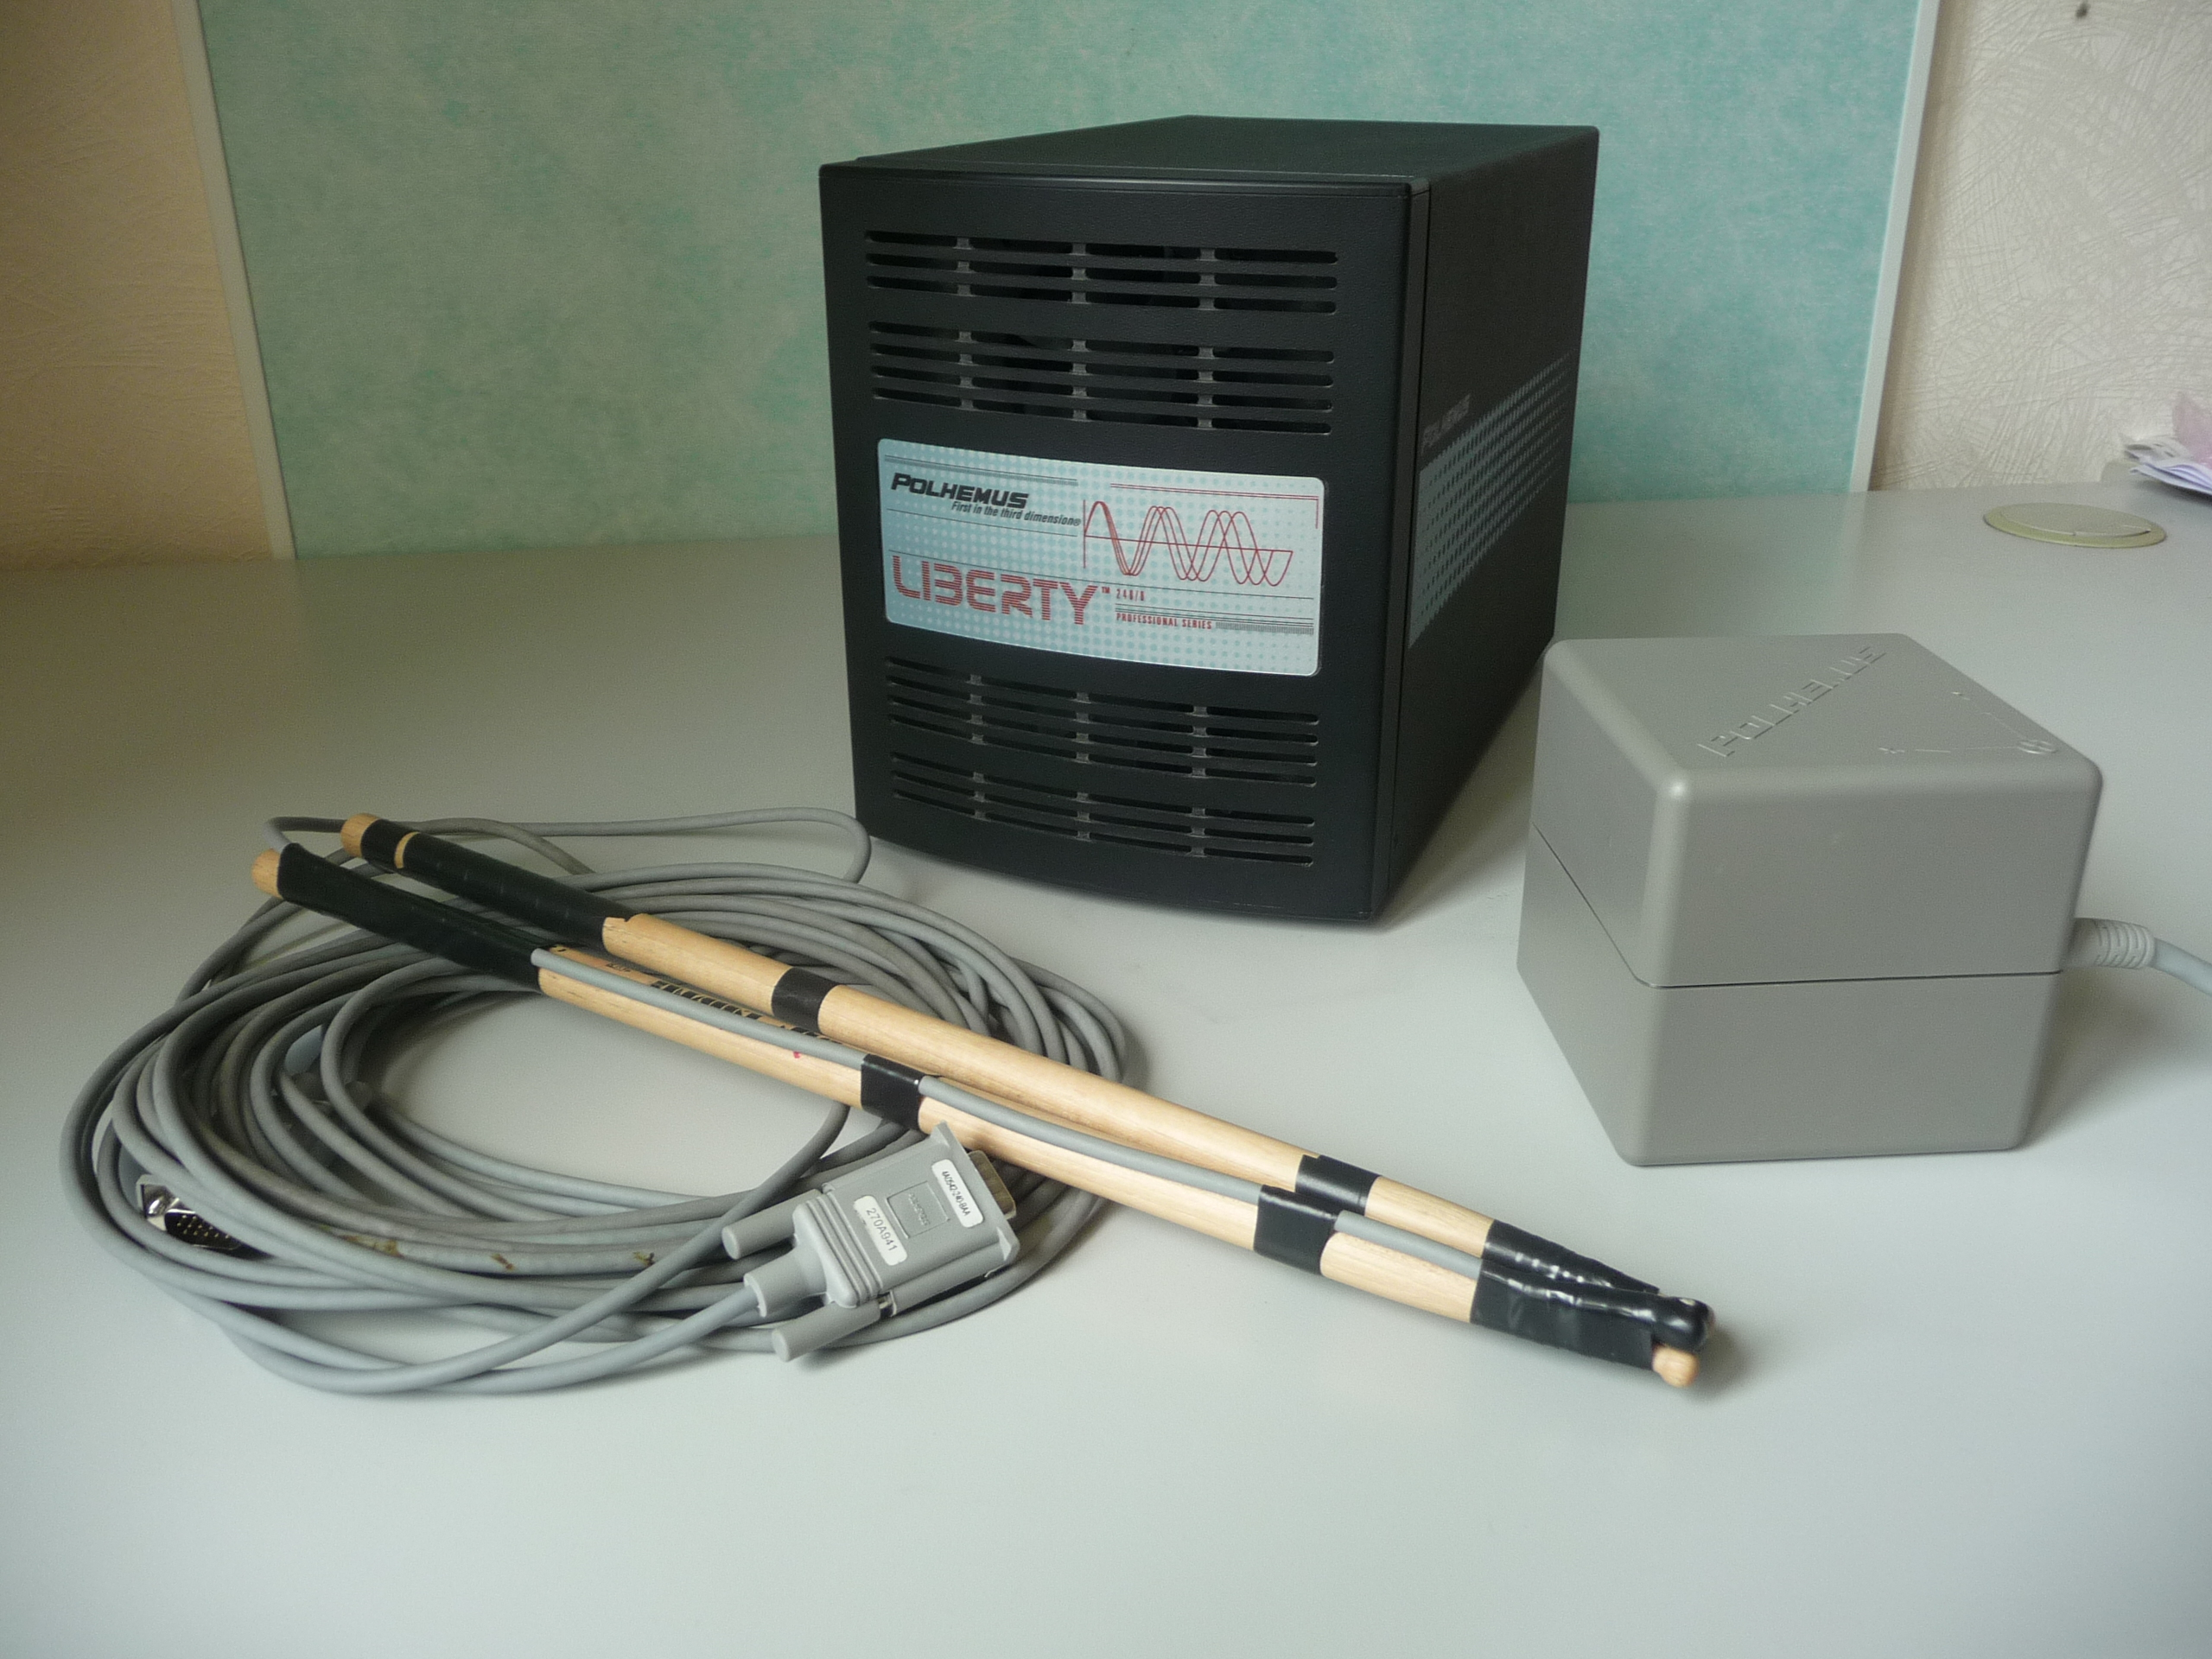
\includegraphics[scale=0.11]{image/percu.jpg}
\caption{Polhemus Liberty and sticks.}
\label{fig:percu}
\end{figure}

However the device is not sufficient on its own, there is also a software part.

\newpage
\subsection{Software: SetKreator and Flock of Birds}
\subsubsection{Flock of Birds}
\ac{FoB} is a small software which receives Polhemus data through the  local network and generates an \ac{OSC} network stream from it.
\ac{OSC} is then easier to manipulate using \brand{MAX/MSP}, \brand{Puredata}, or \brand{OpenFrameworks}.

\subsubsection{SetKreator}
SetKreator has been developed at the \ac{SCRIME} by Joseph Larralde and Sébastien Lebreton. It is a virtual instrument editor for the aerial percussion. Basic volumes (parallelepipeds, cylinders\dots ) inside a sphere which indicates the volume where the Polhemus sensors can be used, like in figure \ref{fig:setkreator}. It is also able to associate each shape to a particular sound synthesis system. It receives position data from the Polhemus via an \ac{OSC} stream.

\begin{figure}[h!]
\centering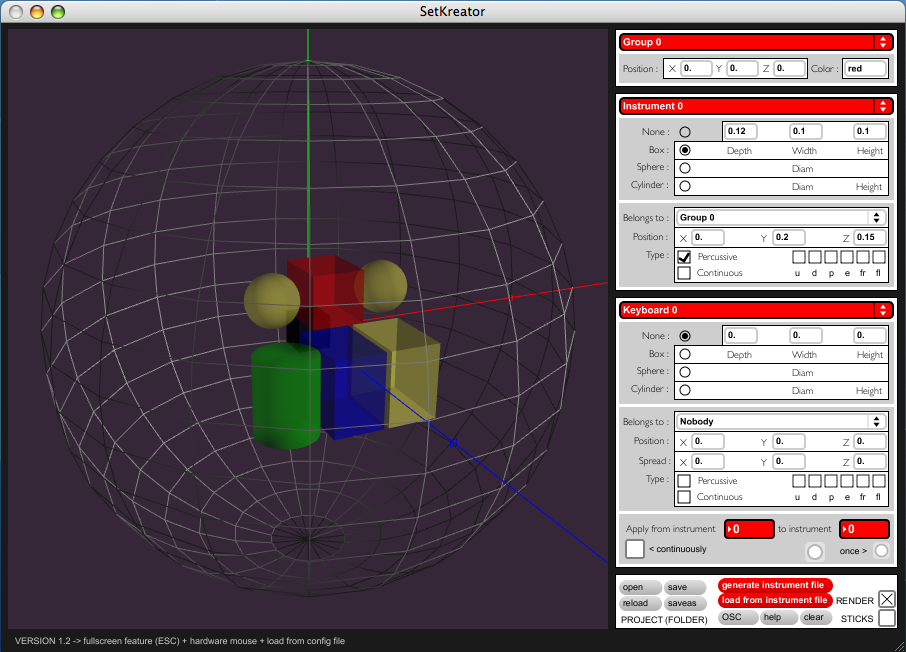
\includegraphics[scale=0.3]{image/setkreator.png}
\caption{SetKreator}
\label{fig:setkreator}
\end{figure}
